\documentclass[tikz,border=12pt]{standalone}
\usepackage[T1]{fontenc}
\usepackage{mathpazo}
\usepackage{amsmath,amssymb}
\usetikzlibrary{arrows.meta, positioning, calc, fit, decorations.pathreplacing}

\definecolor{stblue}{HTML}{7B97AD}
\definecolor{rwgold}{HTML}{B8995E}
\definecolor{sage}{HTML}{7A9A7E}
\definecolor{dkbrown}{HTML}{3D3530}
\definecolor{wmgray}{HTML}{7B7067}
\definecolor{cream}{HTML}{F9F6F0}
\definecolor{border}{HTML}{D4C9B8}
\definecolor{terracotta}{HTML}{C47A6A}
\definecolor{lavender}{HTML}{907EA0}

\begin{document}
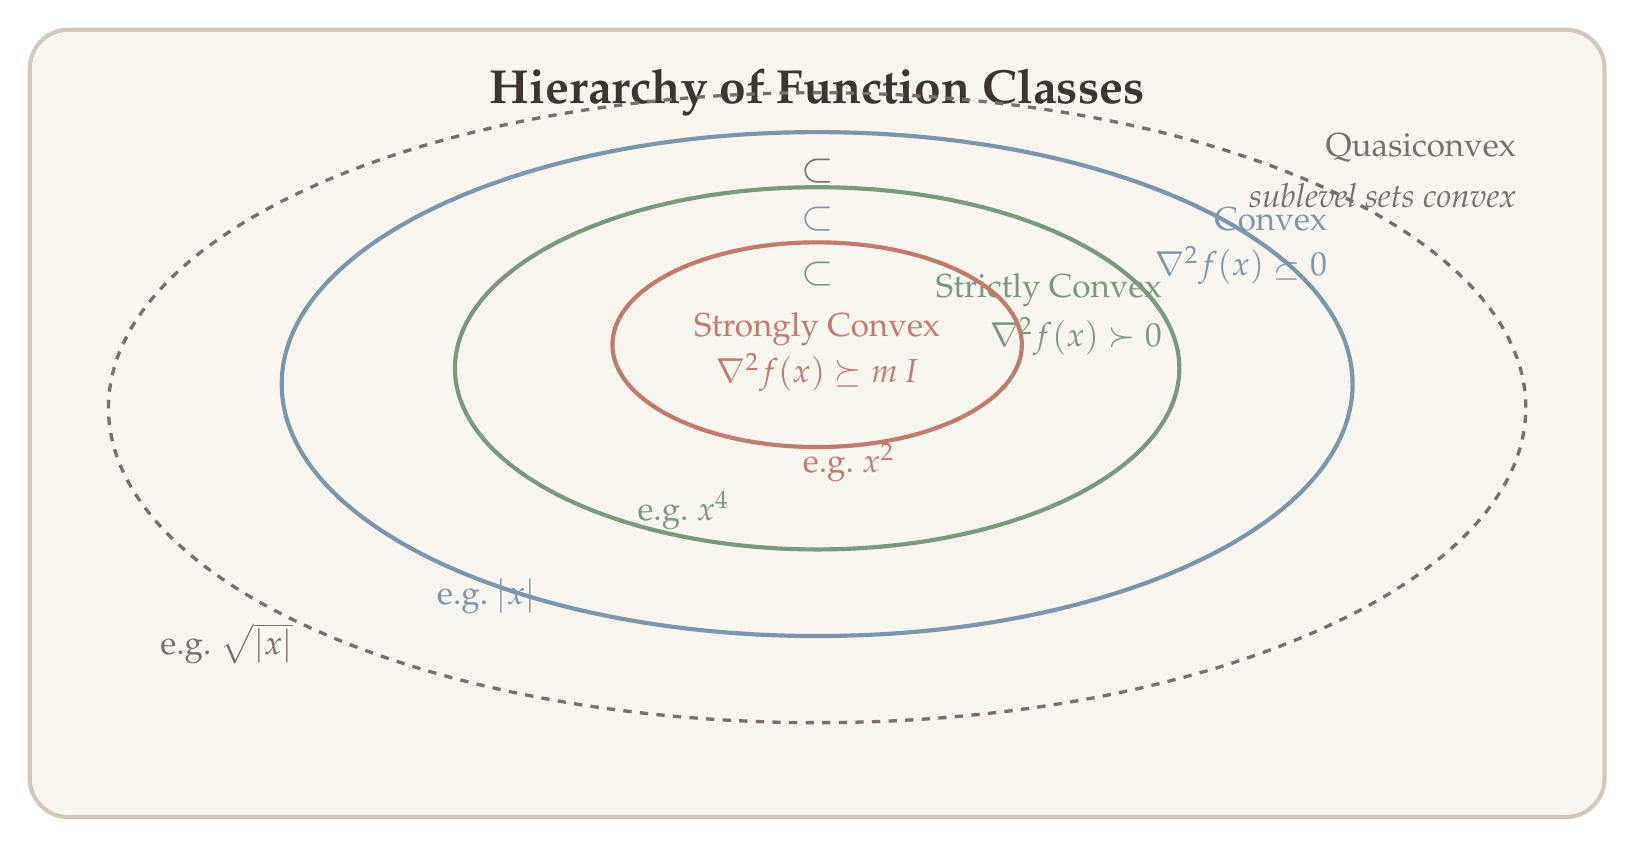
\begin{tikzpicture}[
  every node/.style={text=dkbrown, font=\large},
]

% Background
\fill[cream, rounded corners=14pt] (-10,-6.0) rectangle (10,4.0);
\draw[border, line width=1.5pt, rounded corners=14pt] (-10,-6.0) rectangle (10,4.0);

% Title
\node[font=\LARGE\bfseries, text=dkbrown] at (0,3.2) {Hierarchy of Function Classes};

% Outermost ellipse: Quasiconvex
\draw[wmgray, line width=1.2pt, dashed] (0,-0.8) ellipse (9.0cm and 4.0cm);
\node[font=\large, text=wmgray, anchor=east] at (9.0,2.5) {Quasiconvex};
\node[font=\large\itshape, text=wmgray, anchor=east] at (9.0,1.9) {sublevel sets convex};

% Convex
\draw[stblue, line width=1.5pt] (0,-0.5) ellipse (6.8cm and 3.2cm);
\node[font=\large, text=stblue, anchor=east] at (6.6,1.6) {Convex};
\node[font=\large\itshape, text=stblue, anchor=east] at (6.6,1.0) {$\nabla^2 f(x) \succeq 0$};

% Strictly Convex
\draw[sage, line width=1.5pt] (0,-0.3) ellipse (4.6cm and 2.3cm);
\node[font=\large, text=sage, anchor=east] at (4.5,0.7) {Strictly Convex};
\node[font=\large\itshape, text=sage, anchor=east] at (4.5,0.1) {$\nabla^2 f(x) \succ 0$};

% Strongly Convex (innermost)
\draw[terracotta, line width=1.5pt] (0,0) ellipse (2.6cm and 1.3cm);
\node[font=\large, text=terracotta] at (0,0.2) {Strongly Convex};
\node[font=\large\itshape, text=terracotta] at (0,-0.35) {$\nabla^2 f(x) \succeq m\,I$};

% Example annotations
\node[font=\large, text=wmgray] at (-7.5,-3.8) {e.g.\ $\sqrt{|x|}$};
\node[font=\large, text=stblue] at (-4.2,-3.2) {e.g.\ $|x|$};
\node[font=\large, text=sage] at (-1.7,-2.1) {e.g.\ $x^4$};
\node[font=\large, text=terracotta] at (0.4,-1.5) {e.g.\ $x^2$};

% Subset symbols
\node[font=\Large, text=wmgray] at (0,2.2) {$\subset$};
\node[font=\Large, text=stblue] at (0,1.6) {$\subset$};
\node[font=\Large, text=sage] at (0,0.9) {$\subset$};

\end{tikzpicture}
\end{document}
